% !TeX encoding = UTF-8
% !TeX spellcheck = en_US
\section{Implementation}
\IEEEPARstart{T}his chapter will clarify the development history, 
discovered bugs and design decisions taken.
Let us first take a look on programs 
which already existed when this project started and 
why they have or have not been used  for KeFaX 
and then go into the implementation details.

\subsection{Using existing compilers / compiler-generators}
C/C++ are very complex programming languages with a lot of disambiguties,
lots of different revisions (e.g. ANSI C, ISO/IEC C99\cite{ISOC99}, C++11) and a 
huge amount of compiler specific extensions
(GNU GCC extensions, etc.). 
The Linux kernel makes use of some of the GNU C extensions.
Therefore, it is not possible to compile the vanilla sources of the Linux kernel with Clang
LLVM yet - the Clang front-end\cite{ClangIntro} would provide a nice abstract syntax tree (AST), 
e.g., as a XML file.
Clang claims to be fully GNU gcc compliant and is
used as a replacement of the GNU compiler suite already in
several projects because of its advanced static code analyzing
capabilities. Part of the function declaration of the main-
function for the hello-world example can be found in code
listing \ref{clangast}.
\lstinputlisting[language=XML, firstline=1, lastline=10,
frame=single,extendedchars=true,label=clangast,caption={part of the clang-ast output file},
breaklines=true,]{code/clang-ast.txt}
Another issue is still that their is only limited support for 
traversing, working and exporting the AST for further investigations
by other applications.

GNU gcc itself provides its internal data structures to external programs.
Applications might use this information and provide AST as XML, e.g.
XOgastan\cite{XOgastan} or 
GCC\_XML \cite{gccxml}.
An example
output for gcc-xml can be seen in source code listing \ref{gccxml}
\lstinputlisting[frame=single,extendedchars=true,label=gccxml,language=XML,
  caption={part of the gccxmloutput.xml file},
  firstline=517, lastline=523,
  breaklines=true,]{code/gccxmloutput.xml}
When at first this method seemed promising, it turned out
that gcc-xml is generating too much non-descriptive IDs, is
sometimes buggy and that the GNU gcc itself is not producing
an easily iterate-able AST itself.
\\ \ \\
Compiler compilers are based on processing formal
grammars. The research in theoretic computer science has led
to the automation of generating scanners and parsers out of an
existing formal description text of the programming language
(wherefore often the EBNF - extended Backus-Naur-Form - is
used as a notation).
For compiler generators like Coco/R\cite{COCOR}
(which has been developed at the SSW
institute at the JKU in Linz), 
GNU's implementation of Yacc called Bison\cite{Bison}, etc. there is no unique 
and/or clear EBNF available for C/C++ which would also include most of the GNU C extensions.
One disadvantage of compiler
compilers is the mixture of multiple languages (one language
for describing the scanning/parsing process mixed with the
source code statements for the resulting compiler). Another
disadvantage is that often C/C++ EBNF descriptions lack
language features like the GNU C extensions or others. But the worst
matter is that all information about preprocessor statements
in C and C++ are lost because EBNFs can not deal with
include or define macros.
EBNF profiles of various programming languages can
be found in the grammarware Github repository\cite{Grammarzoo}.
A little out-dated grammar description 
for GNU GCC can be found at \cite{GNUCEBNF}.
\\ \ \\
The problem with most of the evaluated tools is that they are either 
not available anymore or are out-dated or buggy.
But even if they would work, 
the next question is how to build-up the AST, 
which tools and which data structures to use and 
how much effort would be required to do so \dots

\subsection{Reverse Engineering}
How about using {\it EMF (Eclipse Modeling Framework)}
\cite{Eclipse_EMF}
\cite{steinberg2008emf}
instead? EMF provides rich APIs for processing and transforming 
a model into other models or code.
%An tutorial on EMF can be found at 
% insert LINK here!!!
%
So which projects
exist for working with C/C++ in conjunction with EMF?

\subsubsection{EMF4CPP}
The first hit on Google when searching for EMF and C/C++ is 
{\it EMF4CPP}
\cite{EMF4CPP} 
\cite{senac2010emf4cpp}. 
It provides the ability to work with EMF models inside a 
C++ project
(just like Java is supported out-of-the-box) by including the 
library which is part of EMF4CPP.
Another feature of this open-source project is to enable the 
generation of C++ source text out of an Ecore model.
It also comes with a XText artifact for importing C++ code 
into an EMF model.
Unfortunately, as the goal of EMF4CPP is a different one,
it only supports a small subset of C++, 
e.g. it is not possible to 
use macro directives, embedded C or assembler code.

\subsubsection{Eclipse MoDisco}
So far, the approaches have been disappointing because
every one had major disadvantages. But the method described
in this section about Eclipse MoDisco seems promising.

\begin{figure}[ht]
    \centering
	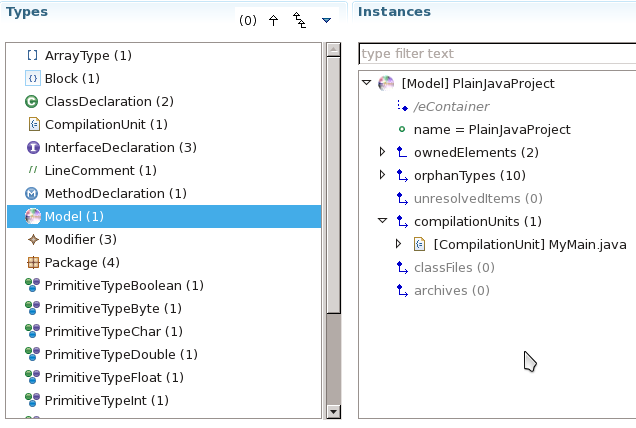
\includegraphics[scale=0.5]{images/JavaAST-2}
	\caption{Eclipse MoDisco model for a simple Java project}
    \label{fig:JavaAST2}
\end{figure}

Inspired by Schneiden et al. "Model-Based Mining of Source Code Repositories"
\cite{scheidgen2014model} the idea came up that it might be interesting to develop
an {\it Eclipse MoDisco discoverer} \cite{Modisco_1}
\cite{bruneliere2010modisco}
\cite{bruneliere2014modisco}.
{\it Eclipse MoDisco} is a reverse-engineering framework which is built on top of the
{\it Eclipse EMF} (Eclipse Modeling Framework)..
This would solve the question of which data structure / abstract syntax tree
to use for storage.
Discoverers are a set of Eclipse plug-ins that provide an importer/parser for a 
certain programming language.
There exist discoverers for Java, JSP, JSON and many more.
Unfortunately, {\it Eclipse MoDisco discoverers} for C and C++ 
did not exist when starting this project.
In the Eclipse forum in a thread called ``Looking for c/c++ discoverer''
\cite{C_Discoverer} it was suggested to piggy-back use {\it Eclipse CDT}
\cite{Eclipse_CDT}\cite{piatov2012using} to implement a C/C++ discoverer.

%\subsection{XText}
%XText is an Eclipse plug-in with which it is possible to design a DSL (domain-specific language).
%With its advanced editors this application allows to import and process DSL artifacts easily
%and re-use the automatically generated models.
%One problem with XText is that it is based on ANTLR and, therefore, can not deal with 
%left recursion. Most C/C++ EBNFs are somehow using left-recursion to simplify the writing.
%Other non-trivial problems can occur too when dealing with rich general-purpose languages like the C
%program family. One try in using XText for parsing C/C++ can be seen below in figure \ref{fig:xtext}.
%\begin{figure}[ht]
%    \centering
%	\includegraphics[scale=0.5]{images/xtext}
%	\caption{Editing a xtext file}
%    \label{fig:xtext}
%\end{figure}
%\FloatBarrier
